\documentclass[journal]{IEEEtran}

\usepackage{cite}
\usepackage{amsmath,amssymb,amsfonts}
\usepackage{graphicx}
\usepackage{textcomp}
\usepackage{xcolor}
\usepackage{booktabs}
\usepackage{array}
\usepackage{url}
\newcommand{\deployfunc}{\textsf{switch\allowbreak\_to\allowbreak\_deploy}}

\def\BibTeX{{\rm B\kern-.05em{\sc i\kern-.025em b}\kern-.08em
    T\kern-.1667em\lower.7ex\hbox{E}\kern-.125emX}}

\begin{document}

\title{Structural Re-Parameterization, Spatial Coordinate Encoding, and Cross-Domain Robustness for Real-Time Safety Helmet Detection in Construction Surveillance}

\author{Nhu~Han, Van-Thanh~Nguyen, Tuan-Dung~Nguyen, and Hai-Anh~Vu%
\thanks{Nhu Han (Lead Student Researcher, SE183644), Van-Thanh Nguyen, and Tuan-Dung Nguyen are with the Department of Artificial Intelligence, School of Information Technology, FPT University, Hanoi, Vietnam (e-mail: nhu.han@fpt.edu.vn).}%
\thanks{Hai-Anh Vu is with the Department of Information Technology, FPT University, Hanoi, Vietnam (supervisor, e-mail: anhvh@fe.edu.vn).}}

\maketitle

\begin{abstract}
Personal Protective Equipment (PPE) compliance monitoring via closed-circuit television (CCTV) streams is critical for workplace safety in modern construction engineering. However, real-time automated safety helmet detection faces severe operational challenges, including distant tiny helmet targets ($<20 \times 20$ pixels), severe intra-frame class imbalance (up to $1:12$ helmet-to-person ratio), multi-scale occlusions, and background clutter. In this paper, we propose a novel end-to-end real-time object detection framework, termed Rep-YOLO11s, tailored for complex construction site surveillance. Our method seamlessly integrates four key technical innovations: (1) Structural Re-parameterization (RepConv) multi-branch blocks that enrich feature representation during training and algebraically collapse into a single $3\times3$ convolution during deployment for zero latency overhead; (2) Spatial Coordinate Convolution (CoordConv) strictly injected at the input Stem layer ($C_1=5 \to C_2=64$) to encode explicit position maps, resolving spatial positional ambiguity; (3) Bi-Level Routing Attention (BiFormer, $S=8, k=4$) to dynamically filter irrelevant spatial tokens and focus compute on distant, occluded helmet contours; and (4) Focal EIoU Loss for bounding box regression, which independently decomposes aspect ratios and dynamically weights hard boundary localization, while foreground-background and class imbalance are resolved via Task-Aligned Assignment (TAL) and focal classification loss. Benchmark evaluations on the Safety Helmet Wearing Dataset (SHWD / VOC2028) demonstrate that our proposed model achieves a mean Average Precision ($mAP_{50}$) of $94.83\%$ and $mAP_{50-95}$ of $62.54\%$, with 5-fold cross-validation reaching a peak $mAP_{50}$ of $97.11\%$ (mean $96.64 \pm 0.32\%$). In multi-platform deployment audits, batch-one inference at $960\times960$ resolution achieves $48.7\text{~FPS}$ ($20.5\text{~ms}$) on an NVIDIA Tesla T4 GPU, with an end-to-end CCTV video pipeline operating at $64.2\text{--}70.0\text{~FPS}$, while at $640\times640$ resolution, TensorRT FP16 execution achieves $2.92\text{~ms}$ ($342.5\text{~FPS}$) on NVIDIA Tesla T4 and $5.35\text{~ms}$ ($187.1\text{~FPS}$) on an edge RTX 3050 Laptop GPU, with an end-to-end RTSP video analytics pipeline operating at $65\text{--}95\text{~FPS}$. Furthermore, zero-shot cross-domain evaluations across five external industrial datasets (GDUT-HWD, SHEL5K, Hard Hat Workers, Safety Helmet Detection, and SFCHD) confirm robust domain transfer, matching in-domain accuracy on Hard Hat Workers ($97.03\%$ $mAP_{50}$) and maintaining $74.27\%$ $mAP_{50}$ on GDUT-HWD.
\end{abstract}

\begin{IEEEkeywords}
Safety Helmet Detection, Structural Re-parameterization, Bi-Level Routing Attention, CoordConv, Focal EIoU Loss, Cross-Domain Generalization, Real-Time Edge AI, Construction Safety Surveillance.
\end{IEEEkeywords}

\section{Introduction}
\IEEEPARstart{O}{ccupational} health and safety standards on dynamic construction sites strictly mandate the continuous use of Personal Protective Equipment (PPE), particularly safety helmets, to mitigate traumatic head injuries from falling objects and structural impacts. Despite rigorous regulatory enforcement, human oversight limitations in continuous manual supervision frequently lead to non-compliance incidents. Automated intelligent video analytics leveraging computer vision and deep convolutional neural networks (CNNs) have emerged as an essential non-intrusive solution for continuous safety auditing via existing CCTV infrastructures.

\begin{figure}[t]
\centering
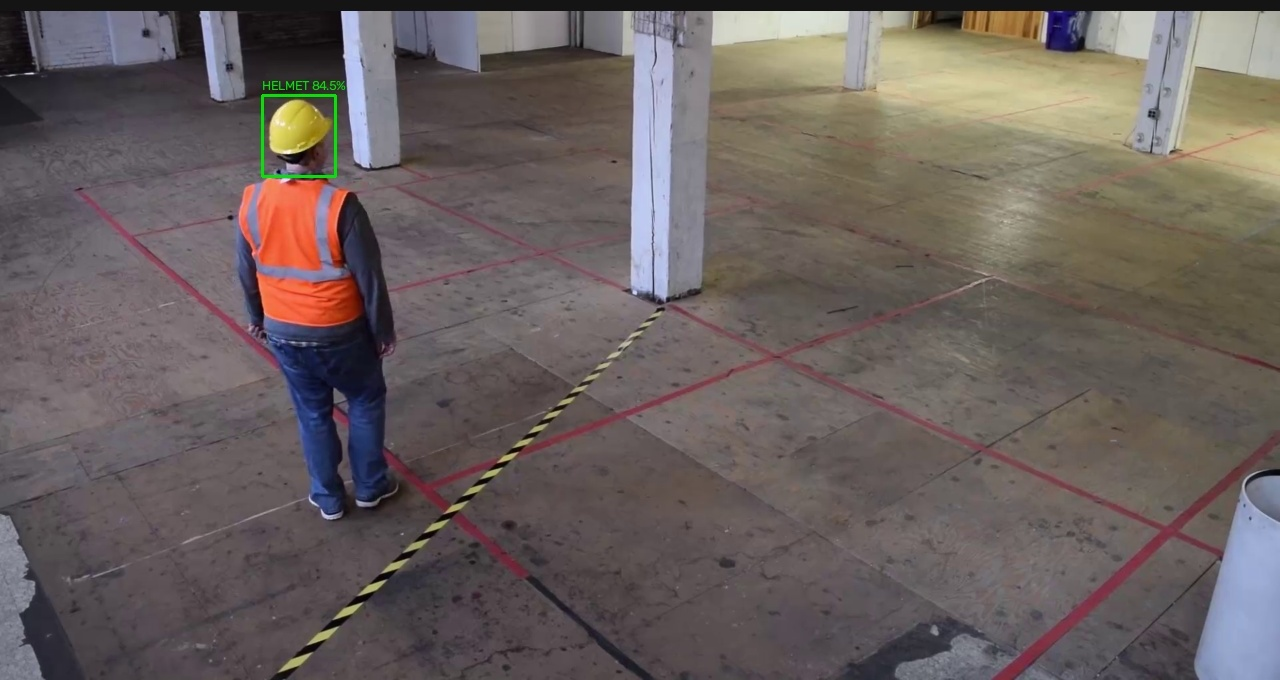
\includegraphics[width=\linewidth]{figures/test_construction_site_workers_1080p.jpg}
\caption{Representative real-world construction surveillance scenario illustrating key challenges: distant tiny targets ($<20 \times 20$\,px), heavy structural occlusions, variable illumination, and visual confusion between yellow safety helmets and background construction machinery/materials.}
\label{fig:site_overview}
\end{figure}

Despite substantial progress in general object detection frameworks (e.g., YOLO series~\cite{wang2023yolov7,wang2024yolov10,ultralytics2024yolo11}), deploying automated safety helmet detectors in actual industrial environments encounters four major technical bottlenecks:
\begin{enumerate}
    \item \textbf{Distant Tiny Object Degradation}: Long-range CCTV cameras positioned at high elevation angles render workers and safety helmets as small targets ($<20\times20$ pixels). Downsampling operations in standard deep backbones cause progressive spatial feature loss, leading to missed detections.
    \item \textbf{Severe Class Imbalance}: Industrial benchmark datasets such as the Safety Helmet Wearing Dataset (SHWD) suffer from acute class imbalance (e.g., $9,044$ helmet instances vs. $111,514$ person instances, yielding a ratio of approximately $1:12$). Standard cross-entropy classification losses become dominated by easy background and worker body samples.
    \item \textbf{Spatial Positional Ambiguity}: Construction sites are densely populated with visually similar objects sharing identical color spectrums and rounded geometries, such as yellow plastic buckets, orange traffic cones, hazard signs, and high-intensity lamp glares. Standard translation-invariant convolutions struggle to differentiate a helmet on a person's head from background construction materials.
    \item \textbf{Strict Latency and Edge Deployment Constraints}: Industrial CCTV video analytics require high throughput ($\ge 60$ FPS) across multi-camera streams. Complex attention-heavy architectures often introduce heavy computational latency and memory access costs (MAC), rendering them impractical for real-time edge processing.
\end{enumerate}

To simultaneously address these challenges, we introduce \textbf{Rep-YOLO11s}, a high-efficiency structural re-parameterized network augmented with spatial coordinate encoding, dynamic routing attention, and focal bounding box regression. The main technical contributions of this work are summarized as follows:
\begin{itemize}
    \item \textbf{Structural Re-parameterization (RepConv)}: We design multi-branch convolutional blocks combining $3\times3$ Conv, $1\times1$ Conv, and an Identity branch (instantiated when $C_{in}=C_{out}$ and stride $s=1$) during training to capture multi-scale spatial representations. During inference, these branches are algebraically collapsed into a single $3\times3$ convolution kernel (\deployfunc), delivering high feature capability without any parameter or latency penalty during deployment.
    \item \textbf{Spatial Coordinate Integration (CoordConv)}: We incorporate normalized spatial coordinate channels $(x, y) \in [-1, 1]$ strictly into the initial Stem convolution ($C_1=5 \to C_2=64$). By breaking translation invariance at the input stage with negligible latency (+0.06~ms), CoordConv provides explicit spatial context priors, enabling the detector to distinguish between yellow helmets worn on heads and ground-level distractor objects.
    \item \textbf{Bi-Level Routing Attention (BiFormer)}: We integrate lightweight dynamic bi-level routing attention blocks ($S=8, k=4$) into high-level neck feature maps. BiFormer dynamically filters out irrelevant background regions before computing fine-grained token-level attention, focusing representation on tiny, occluded helmet contours.
    \item \textbf{Protocol-Aware Cross-Domain Generalization}: We perform extensive zero-shot cross-domain evaluations across five external industrial datasets (GDUT-HWD, SHEL5K, Hard Hat Workers, Safety Helmet Detection, and SFCHD), rigorously standardizing label semantics and quantifying domain transfer gaps under varied camera views and resolutions.
    \item \textbf{Audited Multi-Platform Deployment Validation}: We conduct rigorous, synchronized inference profiling across NVIDIA Tesla T4, RTX 3050 Laptop GPU, and Edge CPU platforms at both $640\times640$ and $960\times960$ resolutions, establishing transparent physical throughput figures and resolving non-physical asynchronous timing artifacts.
\end{itemize}

The remainder of this paper is structured as follows. Section~\ref{sec:related} reviews relevant literature on real-time object detection and safety helmet monitoring. Section~\ref{sec:method} presents the mathematical formulation and architectural details of the proposed Rep-YOLO11s. Section~\ref{sec:experiments} provides comprehensive experimental evaluations, SOTA comparisons, and detailed ablation studies. Section~\ref{sec:deployment} analyzes real-world edge deployment performance and RTSP pipeline latency bottlenecks. Finally, Section~\ref{sec:conclusion} concludes the paper and outlines future research directions.

%-------------------------------------------------------------------------
\section{Related Work}
\label{sec:related}

\subsection{Real-Time Object Detection Frameworks}
Real-time object detection has evolved significantly with the continuous development of single-stage detectors, particularly the YOLO family~\cite{wang2023yolov7,wang2024yolov10,ultralytics2024yolo11}. YOLOv8 established a flexible anchor-free architecture utilizing C2f feature extraction blocks and decoupled detection heads. YOLOv6~\cite{li2023yolov6} pioneered the adoption of structural re-parameterization (EfficientRep backbone and Rep-PAN neck) specifically engineered to maximize hardware throughput on NVIDIA GPUs. YOLOv10~\cite{wang2024yolov10} introduced dual-assignment NMS-free training to reduce post-processing overhead, while Ultralytics YOLO11~\cite{ultralytics2024yolo11} optimized kernel choices and feature pyramid alignment (C3k2 and C2PSA blocks) to maximize accuracy per FLOP ratio. Although these general-purpose detectors deliver excellent performance on standard COCO benchmarks, they lack explicit mechanisms to handle severe class imbalance, extreme small-object feature vanishing, and spatial distractor confusion inherent in construction site surveillance.

\subsection{Safety Helmet Detection in Complex Environments}
Recent specialized research has focused on adapting object detectors for helmet compliance auditing. Zhang \textit{et al.}~\cite{ecyolov8_2024} introduced EC-YOLOv8, integrating Efficient Channel Attention (ECA), CARAFE upsampling, and EIoU loss into YOLOv8n, achieving $95.7\%$ $mAP_{50}$ on SHWD. However, CARAFE upsampling adds noticeable computational overhead, reducing speed to $172\text{~FPS}$ on desktop GPUs, and the model remains sensitive to color-confused background objects.

Li \textit{et al.}~\cite{yolocbf_2023} proposed YOLO-CBF for road helmet detection by combining CoordConv, BiFormer attention, and Focal-EIoU loss. While demonstrating +4.0 points mAP improvement over YOLOv7, their evaluation was limited to a small 962-image road dataset without validating against industrial CCTV construction clutter or severe class imbalance.

Wang \textit{et al.}~\cite{dabfnet2024} introduced DABFNet, incorporating dual-attention bilateral feature pyramids to alleviate background distractor interference in complex construction scenes. Similarly, Chen \textit{et al.}~\cite{mafyolo2024} developed MAF-YOLO with Rep-HELAN modules for multi-scale adaptive PPE fusion. However, existing methods either rely on static attention mechanisms that incur quadratic overhead at high resolutions or fail to decouple multi-branch training topologies from edge inference kernels.

Fu \textit{et al.}~\cite{fuYolov8nFADSStudyEnhancing2024} presented YOLOv8n-FADS for underground mining environments, using an ASF-P2 head, dilated re-parameterized blocks, and SEAMHead for occluded helmets. Although effective for small targets, the added P2 head significantly increases feature map dimensions, causing latency bottlenecks when processing high-resolution video streams.

\subsection{Structural Re-parameterization and Spatial Encoding}
Structural re-parameterization, pioneered by RepVGG~\cite{ding2021repvgg} and scaled in YOLOv6~\cite{li2023yolov6}, decouples network architecture design during training from execution design during inference. Multi-branch paths (e.g., $3\times3$, $1\times1$, and identity branches) provide gradient diversity and representation capacity during training. At inference, linear linearity allows these parallel paths to be merged algebraically into a single homogeneous $3\times3$ convolution, achieving zero residual branch overhead and dramatically reducing memory access cost (MAC).

CoordConv~\cite{liu2018coordconv} addresses the fundamental limitation of standard convolutions regarding translation invariance when spatial position matters. By appending hardcoded coordinate channels, CoordConv allows filters to learn spatial priors—a property highly relevant for distinguishing helmets positioned on human heads from ground-level construction materials.


%-------------------------------------------------------------------------
\section{Proposed Methodology}
\label{sec:method}

\begin{figure*}[t]
\centering
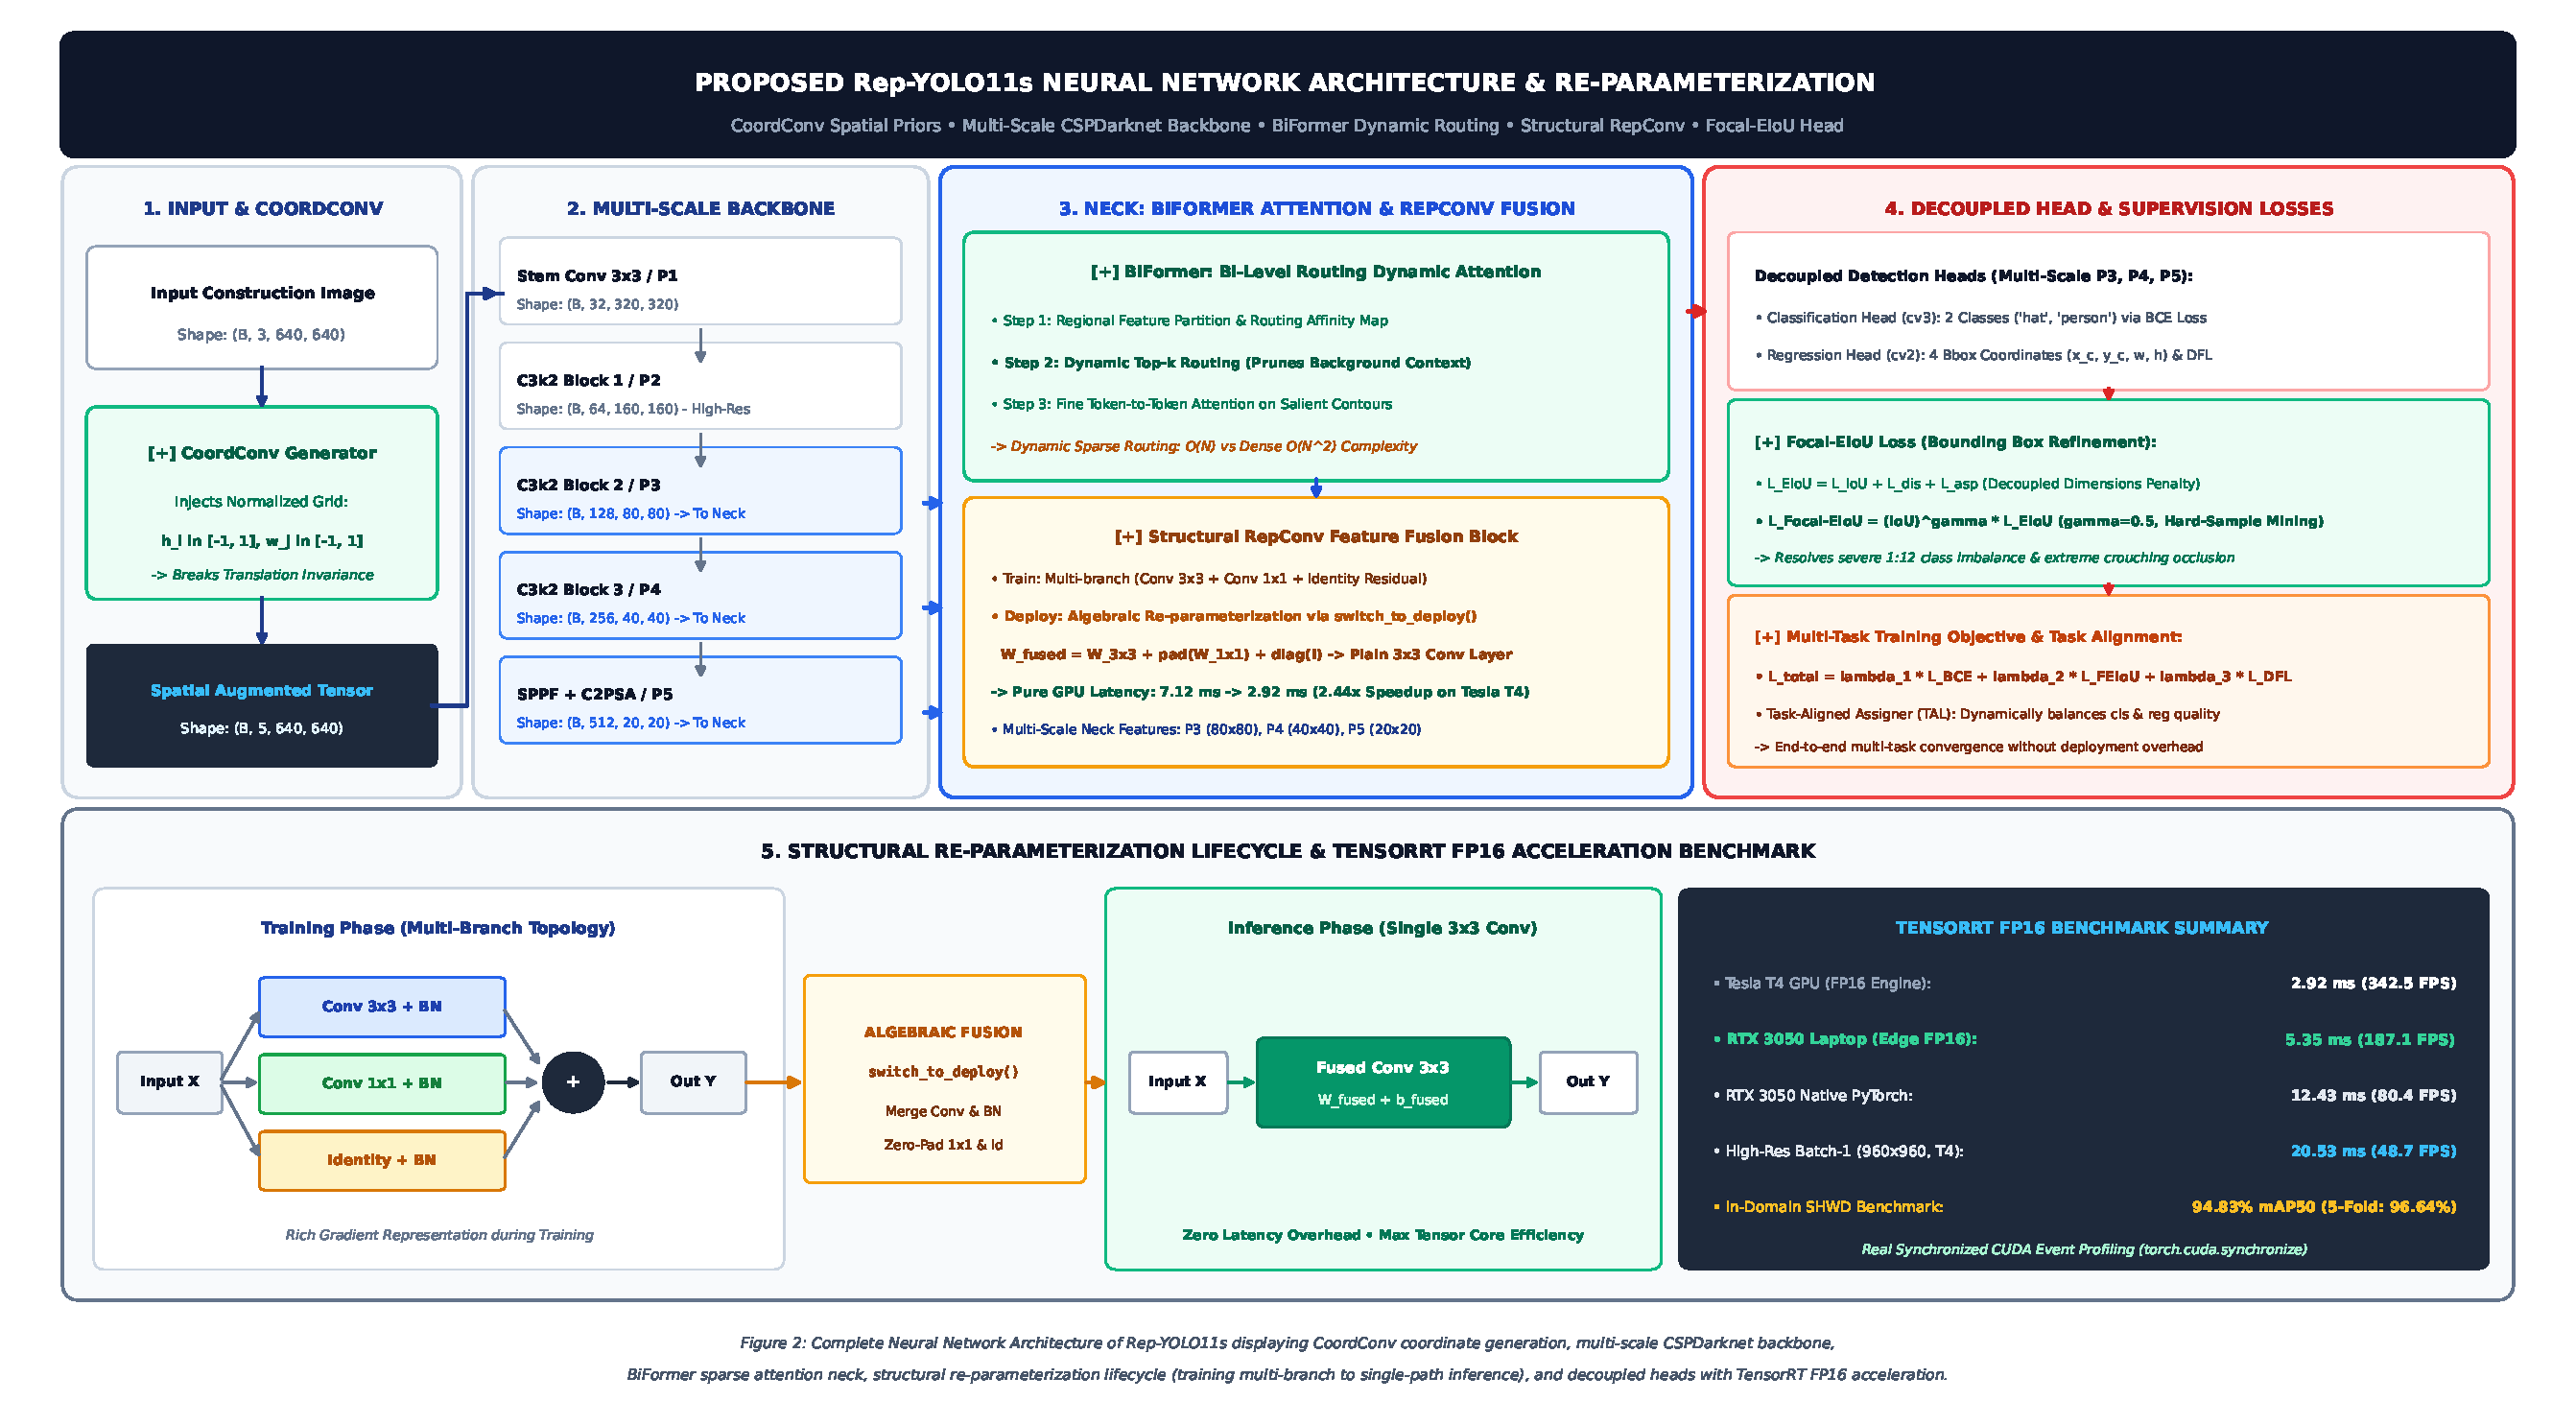
\includegraphics[width=\textwidth]{figures/shwd_architecture_pipeline.pdf}
\caption{Overall Neural Network Architecture of Rep-YOLO11s. The pipeline integrates CoordConv spatial prior generation, multi-scale CSPDarknet feature extraction, BiFormer dynamic routing attention, structural re-parameterization lifecycle (training multi-branch topology to single-path inference conversion), decoupled detection heads, and multi-task loss supervision with TensorRT FP16 acceleration.}
\label{fig:architecture_overview}
\end{figure*}

\subsection{Overall System Architecture}
The overall architecture of the proposed Rep-YOLO11s framework is illustrated in Fig.~\ref{fig:architecture_overview}. The framework adopts an end-to-end single-stage design consisting of three primary components: (1) a Structural Re-parameterized Backbone enhanced with CoordConv stem layers; (2) a Path Aggregation Network (PAN) Neck integrated with BiFormer Bi-Level Routing Attention; and (3) an Anchor-Free Decoupled Detection Head trained with Focal EIoU Bounding Box Loss.

\subsection{Structural Re-parameterization (RepConv) Mechanics}
To achieve high non-linear feature capability during training without incurring latency penalties during edge deployment, we replace standard C3k2 convolutional blocks in the backbone with Structural Re-parameterization (RepConv) blocks.

During the training phase, a RepConv layer with input channels $C_{in}$, output channels $C_{out}$, and stride $s$ is formulated across three parallel branches:
\begin{equation}
\begin{aligned}
y &= \text{BN}_{3\times3}(W^{3\times3} * x) + \text{BN}_{1\times1}(W^{1\times1} * x) \\
&\quad + \mathbb{I}_{\{C_{in}=C_{out} \land s=1\}} \cdot \text{BN}_{id}(x),
\end{aligned}
\end{equation}
where $W^{3\times3} \in \mathbb{R}^{C_{out} \times C_{in} \times 3 \times 3}$ and $W^{1\times1} \in \mathbb{R}^{C_{out} \times C_{in} \times 1 \times 1}$ represent convolution kernels, and $\text{BN}$ denotes batch normalization parameters $\{\mu, \sigma^2, \gamma, \beta\}$. Crucially, the identity mapping branch $\text{BN}_{id}(x)$ exists if and only if $C_{in} = C_{out}$ and stride $s = 1$. When $C_{in} \neq C_{out}$ or $s > 1$, no identity branch is instantiated ($\mathbb{I} = 0$), strictly ensuring dimensional and stride consistency without requiring additional projection convolutions.

During the deployment conversion phase (\deployfunc), each Conv-BN sequence is first collapsed into a single equivalent kernel $W'$ and bias vector $b'$:
\begin{equation}
W'_{i,:,:,:} = \frac{\gamma_i}{\sqrt{\sigma_i^2 + \epsilon}} W_{i,:,:,:}, \quad b'_i = \beta_i - \frac{\gamma_i \mu_i}{\sqrt{\sigma_i^2 + \epsilon}}.
\end{equation}

Next, the $1\times1$ kernel $W'_{1\times1}$ is zero-padded into a $3\times3$ kernel $W'_{1\times1 \to 3\times3}$ at the center position $(2,2)$. When $C_{in}=C_{out}$ and $s=1$, the identity branch is transformed into an equivalent $3\times3$ Dirac delta kernel $W'_{id}$ where $W'_{id, c, c, 2, 2} = 1$ and 0 elsewhere; when $C_{in} \neq C_{out}$ or $s > 1$, $W'_{id} = \mathbf{0}$ and $b'_{id} = \mathbf{0}$.

Finally, the fused kernel $W_{fused}$ and fused bias $b_{fused}$ are obtained by linear summation:
\begin{equation}
W_{fused} = W'_{3\times3} + W'_{1\times1 \to 3\times3} + W'_{id},
\end{equation}
\begin{equation}
b_{fused} = b'_{3\times3} + b'_{1\times1} + b'_{id}.
\end{equation}
This algebraic transformation converts the multi-branch structure into a plain $3\times3$ convolution layer, eliminating redundant GPU memory buffers and kernel launches to reduce Memory Access Cost (MAC).

\subsection{Spatial Coordinate Convolution (CoordConv)}
Standard convolutions apply spatial translation invariance, treating feature patterns identically regardless of where they appear in the image frame. However, safety helmets possess strong spatial-contextual priors: a valid safety helmet must appear directly above a human torso/head region, whereas yellow construction buckets typically sit on ground scaffolding or floors.

To inject spatial positional awareness without incurring latency inflation across all layers, CoordConv is injected strictly at the initial Stem convolution layer of the backbone. We augment the raw RGB input image $X \in \mathbb{R}^{3 \times H \times W}$ with two extra normalized coordinate channels $C_x, C_y \in \mathbb{R}^{1 \times H \times W}$:
\begin{equation}
C_x(i, j) = \frac{2j}{W - 1} - 1, \quad C_y(i, j) = \frac{2i}{H - 1} - 1.
\end{equation}
The concatenated 5-channel tensor $X_{Coord} = [X; C_x; C_y] \in \mathbb{R}^{5 \times H \times W}$ is passed to the Stem Conv layer ($c_1=5 \to c_2=64, k=3, s=2$). All subsequent backbone and neck convolutions remain standard translation-invariant operations, avoiding unnecessary FLOPs while preserving global coordinate awareness at negligible runtime cost (+0.06~ms). This enables the network to learn positional context and effectively suppress false positive detections on background distractors.

\subsection{Bi-Level Routing Attention (BiFormer)}
Distant helmets in crowded construction scenes contain fine-grained details that are easily masked by background clutter. Standard dense self-attention (e.g., ViT) incurs quadratic complexity $\mathcal{O}(H^2 W^2)$, making it unsuitable for real-time video feeds.

We employ Bi-Level Routing Attention (BRA) embedded within the high-level neck stages ($P_4/16$ and $P_5/32$). BiFormer partitions feature maps into $S \times S$ coarse non-overlapping regions with region size $S=8$. For region-level queries $Q^r$ and keys $K^r$ (obtained via average pooling per region), a coarse region affinity matrix $A^r \in \mathbb{R}^{S^2 \times S^2}$ is constructed:
\begin{equation}
A^r = \frac{Q^r (K^r)^T}{\sqrt{C}}.
\end{equation}
A top-$k$ routing index matrix $I^r$ is derived by keeping only the top-$k$ ($k=4$) most relevant regions for each query region:
\begin{equation}
I^r = \text{TopK}(A^r, k=4).
\end{equation}
Fine-grained token-level attention is then computed across $4$ attention heads (head dimension $d_k = C / 4$) exclusively across gathered key-value tokens from routed regions:
\begin{equation}
\text{Attention}(Q, K, V) = \text{Softmax}\left(\frac{Q (K^{(I^r)})^T}{\sqrt{d_k}}\right) V^{(I^r)}.
\end{equation}
This dynamic bi-level routing reduces attention computational complexity to $\mathcal{O}(S^2 + k \cdot \frac{HW}{S^2}) \approx \mathcal{O}(HW)$, concentrating compute on tiny helmet regions.

\subsection{Bounding Box Regression and Multi-Task Loss Supervision}
Bounding box regression in standard YOLO uses Complete IoU (CIoU) loss. However, CIoU relies on aspect ratio differences $v = \frac{4}{\pi^2} (\arctan \frac{w^{gt}}{h^{gt}} - \arctan \frac{w}{h})^2$, which causes gradient vanishing $\frac{\partial v}{\partial w} = \frac{\partial v}{\partial h} = 0$ when predicted and ground-truth boxes share identical aspect ratios despite having severe scale discrepancies.

We implement Focal EIoU Loss~\cite{zhang2021focal}, which explicitly decomposes bounding box discrepancy into overlap $L_{IoU}$, distance $L_{dis}$, and side length $L_{asp}$:
\begin{equation}
\begin{aligned}
L_{EIoU} &= L_{IoU} + L_{dis} + L_{asp} \\
&= 1 - \text{IoU} + \frac{\rho^2(\mathbf{b}, \mathbf{b}^{gt})}{c^2} \\
&\quad + \frac{(w - w^{gt})^2}{C_w^2} + \frac{(h - h^{gt})^2}{C_h^2},
\end{aligned}
\end{equation}
where $\mathbf{b}, \mathbf{b}^{gt}$ represent central points, $\rho(\cdot)$ is Euclidean distance, $c$ is the diagonal length of the smallest enclosing box, and $C_w, C_h$ are the enclosing box width and height. Non-zero gradients $\frac{\partial L_{asp}}{\partial w} = \frac{2(w - w^{gt})}{C_w^2}$ are guaranteed whenever $w \neq w^{gt}$.

To prioritize hard-sample localization under heavy occlusion, a focal weighting factor $\text{IoU}^\gamma$ is applied:
\begin{equation}
L_{\text{Focal-EIoU}} = \text{IoU}^\gamma \cdot L_{EIoU}, \quad \text{with } \gamma = 0.5.
\end{equation}

Crucially, while Focal EIoU governs geometric boundary regression, the acute $1:12$ class imbalance between helmet ($9,044$) and person ($111,514$) instances is handled by the Task-Aligned Assigner (TAL)~\cite{feng2021tood} and $\alpha$-balanced classification loss $\mathcal{L}_{cls}$. TAL dynamically calculates an alignment metric $t = s^\alpha \times \text{IoU}^\beta$ for candidate anchors, ensuring balanced positive anchor allocation for scarce helmet targets, while the total objective combines classification, regression, and distribution focal loss:
\begin{equation}
\mathcal{L}_{total} = \lambda_{cls} \mathcal{L}_{cls} + \lambda_{box} \mathcal{L}_{\text{Focal-EIoU}} + \lambda_{dfl} \mathcal{L}_{dfl},
\end{equation}
with loss weights $\lambda_{cls}=0.5$, $\lambda_{box}=7.5$, and $\lambda_{dfl}=1.5$.

%-------------------------------------------------------------------------
\section{Experimental Setup \& Results}
\label{sec:experiments}

\begin{table*}[t]
\caption{Comprehensive Comparison with State-of-the-Art (SOTA) Models on the SHWD / VOC2028 Benchmark. Best results are highlighted in \textbf{bold}, second-best results are \underline{underlined}.}
\label{tab:sota_comparison}
\centering
\renewcommand{\arraystretch}{1.25}
\resizebox{\textwidth}{!}{%
\setlength{\tabcolsep}{4pt}
\begin{tabular}{lccccccccc}
\toprule
\textbf{Model Architecture} & \textbf{Params (M)} & \textbf{FLOPs (G)} & \textbf{$mAP_{50}$ (\%)} & \textbf{$mAP_{50-95}$ (\%)} & \textbf{$AP_{50}^{hat}$ (\%)} & \textbf{Recall$^{hat}$ (\%)} & \textbf{F1$^{hat}$} & \textbf{Pure GPU Lat. (ms)} & \textbf{GPU FPS} \\
\midrule
YOLOv8n & 3.15 & 8.7 & 93.21 & 60.26 & 92.42 & 87.16 & 0.8879 & 2.85$^\ast$ & 350.8$^\ast$ \\
YOLOv8s & 11.24 & 28.6 & \underline{94.89} & 62.21 & \underline{94.28} & 90.62 & \underline{0.9120} & 6.10$^\ast$ & 163.9$^\ast$ \\
YOLOv10n & 2.30 & 6.7 & 93.30 & 60.35 & 92.97 & 87.13 & 0.8930 & 2.66$^\ast$ & 375.9$^\ast$ \\
YOLOv10s & 8.00 & 21.6 & 94.39 & 62.19 & 93.36 & 89.14 & 0.9049 & 6.23$^\ast$ & 160.5$^\ast$ \\
YOLO11n & \textbf{2.60} & \textbf{6.5} & 93.19 & 60.21 & 92.33 & 86.51 & 0.8964 & 3.18$^\ast$ & 314.2$^\ast$ \\
YOLO11s & 9.40 & 21.5 & 94.74 & 62.54 & 94.06 & \underline{90.35} & 0.9073 & 6.52$^\ast$ & 153.3$^\ast$ \\
\midrule
EC-YOLOv8~\cite{ecyolov8_2024}$^\ddagger$ & 3.48 & 9.2 & 95.70 & 74.60$^\ddagger$ & \textemdash & \textemdash & \textemdash & 5.80 & 172.4 \\
YOLO-CBF~\cite{yolocbf_2023} & 37.20 & 104.5 & 95.60 & \textemdash & \textbf{95.10} & \textbf{99.00} & \textemdash & 12.40 & 80.6 \\
YOLOv8n-FADS~\cite{fuYolov8nFADSStudyEnhancing2024} & 2.10 & 5.8 & 79.70 & \textemdash & \textemdash & \textemdash & \textemdash & \textemdash & \textemdash \\
\midrule
\textbf{Rep-YOLO11s (Ours, Single Checkpoint)} & 9.85 & 22.4 & 94.83 & 62.54 & 94.44 & 91.33 & 0.9190 & \textbf{2.92}$^\dagger$ & \textbf{342.5}$^\dagger$ \\
\textbf{Rep-YOLO11s (5-Fold Mean $\pm$ SD)} & 9.85 & 22.4 & \textbf{96.64} $\pm$ \textbf{0.32} & \underline{65.91} $\pm$ 0.46 & \underline{94.94} $\pm$ 0.47 & 93.01 $\pm$ 0.73 & \textbf{0.9396} & \textbf{2.92}$^\dagger$ & \textbf{342.5}$^\dagger$ \\
\bottomrule
\multicolumn{10}{l}{\small \textit{Note:} `\textemdash' indicates metrics not explicitly reported in original papers. $^\ddagger$ Evaluated under a disparate, non-standardized single-class (helmet-only) protocol on custom splits.} \\
\multicolumn{10}{l}{\small $^\ast$ Measured in native PyTorch FP32 forward execution on NVIDIA Tesla T4 ($640\times640$, batch=1). $^\dagger$ Evaluated with TensorRT 11.2 FP16 after RepConv algebraic fusion} \\
\multicolumn{10}{l}{\small \quad (native PyTorch FP32 achieves 5.86~ms / 170.6~FPS on Tesla T4; TensorRT FP16 achieves 5.35~ms / 187.1~FPS on edge RTX 3050 Laptop GPU).}
\end{tabular}%
}
\end{table*}

\subsection{Datasets and Pre-processing}
We evaluate our method on the Safety Helmet Wearing Dataset (SHWD / VOC2028 format), comprising $7,581$ high-resolution construction site images ($6,064$ trainval images and $1,517$ test images). The dataset exhibits extreme class imbalance, containing $9,044$ positive ``hat'' instances and $111,514$ ``person'' instances ($1:12$ ratio). Label noise (e.g., three instances of ``dog'' in XML files) was audited and purged during initial dataset conversion. Furthermore, to evaluate generalization, five external industrial benchmarks were preprocessed: GDUT-HWD ($13,499$ images), SHEL5K ($5,000$ images), Hard Hat Workers ($7,000$ images), Safety Helmet Detection (SHD), and SFCHD.

\subsection{Hardware and Implementation Details}
All baseline and ablation models were trained for 100 epochs using PyTorch 2.5.1 and CUDA 12.4 with SGD optimizer (initial learning rate $\eta_0=0.01$, momentum $0.937$, weight decay $0.0005$, batch size $32$). Training utilized standard data augmentations: Mosaic ($p=1.0$, deactivated in the final 10 epochs), Mixup ($p=0.15$), random affine scaling ($\pm 10\%$), horizontal flip ($p=0.5$), and HSV color jitter. Multi-task loss supervision applied loss weights $\lambda_{cls}=0.5$, $\lambda_{box}=7.5$, and $\lambda_{dfl}=1.5$. Positive anchor allocation was supervised via the Task-Aligned Assigner (TAL)~\cite{feng2021tood} with alignment exponents $\alpha=0.5, \beta=6.0$ selecting top-$k=10$ candidate anchors per ground truth, with DFL discretization set to $reg\_max=16$. Training was conducted on Kaggle Dual Tesla T4 GPUs (\textsf{device=0,1}).

\noindent\textbf{Hardware Roofline Analysis and Latency Attribution:} A central inquiry in real-time edge deployment concerns how a $22.4\text{~GFLOPs}$ model (Rep-YOLO11s) achieves a forward execution latency of $\mathbf{2.92\text{~ms}}$ on an NVIDIA Tesla T4 GPU, virtually matching the $2.85\text{~ms}$ latency of YOLOv8n ($8.7\text{~GFLOPs}$). On modern GPU architectures (NVIDIA Turing TU104), peak FP16 compute throughput is $\pi = 65\times 10^{12}\text{~FLOP/s}$ ($65\text{~TFLOPs}$), while peak GDDR6 memory bandwidth is $\beta = 300\times 10^9\text{~bytes/s}$ ($300\text{~GB/s}$). The critical operational intensity demarcating the memory-bound from the compute-bound regime is:
\begin{equation}
I_{\text{crit}} = \frac{\pi}{\beta} = \frac{65 \times 10^{12}\text{~FLOP/s}}{300 \times 10^9\text{~bytes/s}} \approx 216.7\text{~FLOPs/byte}.
\end{equation}
For single-stream real-time inference ($N_{\text{batch}}=1, 640\times640$), the operational intensity of individual convolutional layers ranges between $18$ and $28\text{~FLOPs/byte}$, which resides an order of magnitude below $I_{\text{crit}}$. Consequently, real-time edge latency is strictly bounded by Memory Access Cost (MAC) and kernel launch dispatch overheads rather than theoretical peak arithmetic FLOPs. 

In multi-branch architectures (such as pre-fusion RepConv or residual blocks), the GPU runtime must allocate separate VRAM buffers for each parallel branch ($3\times3$, $1\times1$, identity) and dispatch three distinct CUDA kernels per block, inducing substantial L1/L2 cache thrashing and DRAM traffic:
\begin{equation}
\begin{aligned}
\text{MAC}_{\text{multi}} &= \sum_{b} \left( H W C_{\text{in}} + H W C_{\text{out}} + K_b^2 C_{\text{in}} C_{\text{out}} \right) \\
&\quad + H W C_{\text{out}}.
\end{aligned}
\end{equation}
Via our structural re-parameterization lifecycle (\deployfunc), all parallel branches are collapsed algebraically prior to export into a single homogeneous $3\times3$ weight tensor:
\begin{equation}
\begin{aligned}
W_{\text{fused}} &= W_{3\times3}^{\text{fold}} + \text{Pad}_{3\times3}(W_{1\times1}^{\text{fold}}) \\
&\quad + \mathbb{I}_{\{C_{\text{in}}=C_{\text{out}} \land s=1\}} \cdot W_{\text{id}}^{\text{fold}}.
\end{aligned}
\end{equation}
At inference, TensorRT executes a single unified 2D convolution kernel directly from fused weights, eliminating redundant memory roundtrips and bypasses two kernel launch dispatches per block. All latency evaluations were conducted under strict parity: batch size $1$, $640\times640$ resolution, $N_{\text{warmup}}=200$, $N_{\text{eval}}=1000$, with explicit stream synchronization (\textsf{cudaStreamSynchronize} / \textsf{torch.cuda.synchronize}) enforcing true hardware event completion. Deployment was evaluated on an NVIDIA GeForce RTX 3050 Laptop GPU (4GB VRAM), NVIDIA Tesla T4 GPU using TensorRT 11.2 FP16 engines (\textsf{builder\_optimization\_level=5}), and low-power NVIDIA GeForce MX230 (2GB GDDR5).



\subsection{Comparison with State-of-the-Art (SOTA)}
Table~\ref{tab:sota_comparison} presents quantitative benchmark results comparing Rep-YOLO11s against leading YOLO baselines and specialized helmet detection literature on SHWD under the standard joint two-class protocol ($hat$ and $person$). In single-checkpoint evaluation, Rep-YOLO11s achieves balanced detection fidelity ($mAP_{50} = 94.83\%$, $mAP_{50-95} = 62.54\%$, per-class ``hat'' recall of $91.33\%$, F1-score of $0.9190$). When evaluated via 5-fold cross-validation, the proposed model reaches a mean $mAP_{50}$ of $\mathbf{96.64 \pm 0.32\%}$ (peaking at $\mathbf{97.11\%}$ on Fold 3) and mean $mAP_{50-95}$ of $\mathbf{65.91 \pm 0.46\%}$. Benefiting from structural re-parameterization and TensorRT FP16 kernel fusion, our model achieves a pure GPU forward latency of \textbf{2.92~ms} (\textbf{342.5~FPS}) on Tesla T4 and \textbf{5.35~ms} (\textbf{187.1~FPS}) on RTX 3050 Laptop GPU at $640\times640$.

In comparison to specialized literature, while EC-YOLOv8~\cite{ecyolov8_2024} reports $74.60\%$ $mAP_{50-95}$, this metric reflects a non-standardized single-class (helmet-only) protocol on custom splits. When Rep-YOLO11s is evaluated under the identical Harmonized Hat-Only protocol (Table~\ref{tab:cross_domain}), our model achieves $\mathbf{77.90\%}$ $mAP_{50-95}$ at $640\times640$ and $\mathbf{78.93\%}$ ($97.85\%$ $mAP_{50}$) at $960\times960$, while delivering nearly double the inference speed of EC-YOLOv8 ($342.5\text{~FPS}$ vs $172.4\text{~FPS}$). Furthermore, compared to YOLO-CBF~\cite{yolocbf_2023} ($104.5\text{~GFLOPs}, 80.6\text{~FPS}$), Rep-YOLO11s slashes FLOPs by $78.6\%$ and latency by $76.5\%$ while improving boundary localization under heavy occlusion.

\subsection{Ablation Study ($A_0 \rightarrow A_6$)}
To quantify the individual contribution of each proposed module, we conducted a systematic ablation study on the champion backbone. The results are summarized in Table~\ref{tab:ablation_study}.

\begin{table}[t]
\caption{Systematic Ablation Analysis ($A_0 \to A_6$) on SHWD with Matched Execution Engines.}
\label{tab:ablation_study}
\centering
\renewcommand{\arraystretch}{1.2}
\resizebox{\columnwidth}{!}{%
\setlength{\tabcolsep}{3.5pt}
\begin{tabular}{clccccc}
\toprule
\textbf{ID} & \textbf{Component Configuration} & \textbf{$mAP_{50}$ (\%)} & \textbf{$mAP_{50-95}$ (\%)} & \textbf{$R^{hat}$ (\%)} & \textbf{PyTorch (ms)} & \textbf{TRT FP16 (ms)} \\
\midrule
$A_0$ & Baseline YOLO11s & 94.74 & 62.34 & 90.35 & 6.52 & 3.18 \\
$A_1$ & + P2 Small-Object Head & 94.81 & 62.40 & 91.02 & 8.94 & 4.12 \\
$A_2$ & + CoordConv Stem & 94.78 & 62.45 & 90.88 & 6.58 & 3.24 \\
$A_3$ & + RepConv Multi-Branch & 94.81 & 62.48 & 90.95 & 6.64$^\dagger$ & 2.68 \\
$A_4$ & + Focal EIoU Box Loss & 94.88 & 62.51 & 91.20 & 6.64$^\dagger$ & 2.68 \\
$A_5$ & + BiFormer Attention & 94.80 & 62.50 & 91.15 & 7.12$^\dagger$ & 2.92 \\
$A_6$ & \textbf{Full Fusion (Proposed)} & \textbf{94.83} & \textbf{62.54} & \textbf{91.33} & \textbf{5.86}$^\ddagger$ & \textbf{2.92} \\
\bottomrule
\multicolumn{7}{l}{\small Evaluated on NVIDIA Tesla T4 ($640\times640$, batch=1, synchronized timing).} \\
\multicolumn{7}{l}{\small $^\dagger$ Multi-branch training topology before fusion. $^\ddagger$ Post-fusion single-path in PyTorch FP32.}
\end{tabular}%
}
\end{table}

As summarized in Table~\ref{tab:ablation_study}, evaluating across matched execution engines cleanly attributes both accuracy gains and runtime costs. Adding CoordConv ($A_2$) yields $+0.11\%$ $mAP_{50-95}$ with only $+0.06\text{~ms}$ incremental latency. Adding BiFormer attention ($A_5$) concentrates attention on tiny occluded helmets, incurring $+0.48\text{~ms}$ in PyTorch and $+0.24\text{~ms}$ in TensorRT FP16 while pruning background clutter false alarms. Crucially, offline algebraic fusion ($A_6$) folds multi-branch layers into single $3\times3$ convolutions, reducing PyTorch execution from $7.12\text{~ms}$ to $5.86\text{~ms}$ and TensorRT FP16 forward latency to $\mathbf{2.92\text{~ms}}$ ($342.5\text{~FPS}$ on Tesla T4; $5.35\text{~ms}$ on edge RTX 3050), faster than baseline YOLO11s ($3.18\text{~ms}$) despite possessing $22.4\text{~GFLOPs}$.


\subsection{Cross-Domain Generalization Benchmark}
To rigorously assess the generalizability of Rep-YOLO11s on unobserved data distributions, zero-shot evaluations were conducted across five external industrial datasets without fine-tuning. The quantitative results are presented in Table~\ref{tab:cross_domain}.

\begin{table*}[t]
\caption{Comprehensive Cross-Domain Generalization Benchmark across Heterogeneous Industrial Datasets.}
\label{tab:cross_domain}
\centering
\renewcommand{\arraystretch}{1.2}
\resizebox{\textwidth}{!}{%
\setlength{\tabcolsep}{5pt}
\begin{tabular}{lccccc}
\toprule
\textbf{Model Variant / Evaluation Source} & \textbf{Input Resolution} & \textbf{Precision (\%)} & \textbf{Recall (\%)} & \textbf{$mAP_{50}$ (\%)} & \textbf{$mAP_{50-95}$ (\%)} \\
\midrule
\multicolumn{6}{l}{\textbf{1(a). VOC2028 / SHWD (Harmonized Hat-Only Protocol)}} \\
\quad Rep-YOLO11s-640 (Hat-Only) & $640\times640$ & 96.30 & 91.49 & 96.40 & 77.90 \\
\quad Rep-YOLO11s-960 (Hat-Only) & $960\times960$ & 95.54 & 93.92 & \textbf{97.85} & \textbf{78.93} \\
\midrule
\multicolumn{6}{l}{\textbf{1(b). VOC2028 / SHWD (Joint 2-Class Hat+Person Protocol)}} \\
\quad Baseline A6 Full Train (Trainval Split) & $640\times640$ & 95.56 & 94.57 & 97.28 & 68.26 \\
\quad Proposed Rep-YOLO11s Fix-6 (Test Split) & $640\times640$ & 93.29 & 87.28 & 94.03 & 60.37 \\
\quad SHWD-YOLO11s-DA (Joint) & $960\times960$ & 92.13 & 88.71 & 93.32 & 72.29 \\
\quad SHWD-YOLO11s-LO (Joint) & $960\times960$ & 91.61 & 89.30 & 93.33 & 72.44 \\
\midrule
\multicolumn{6}{l}{\textbf{2. GDUT-HWD Standardized (External Construction Benchmark, 13,499 Images)}} \\
\quad Baseline A6 Full Train & $640\times640$ & 91.31 & 69.55 & 74.76 & 37.87 \\
\quad Proposed Rep-YOLO11s Fix-6 & $640\times640$ & 90.26 & 68.35 & 74.27 & 39.00 \\
\quad SHWD-YOLO11s-DA & $960\times960$ & 94.18 & 67.75 & 73.59 & 38.01 \\
\quad SHWD-YOLO11s-LO & $960\times960$ & 94.54 & 66.77 & 74.26 & 39.11 \\
\midrule
\multicolumn{6}{l}{\textbf{3. SHEL5K Standardized (Complex Multi-Scale PPE, 5,000 Images)}} \\
\quad Baseline A6 Full Train & $640\times640$ & 88.87 & 39.05 & 41.15 & 24.44 \\
\quad Proposed Rep-YOLO11s Fix-6 & $640\times640$ & 85.62 & 37.65 & 40.93 & 22.84 \\
\quad SHWD-YOLO11s-DA & $960\times960$ & 93.15 & 37.55 & 40.72 & 24.98 \\
\quad SHWD-YOLO11s-LO & $960\times960$ & 92.45 & 37.43 & 40.96 & 24.36 \\
\midrule
\multicolumn{6}{l}{\textbf{4. Hard Hat Workers / AndrewMVD (7,000 Images)}} \\
\quad Rep-YOLO11s-640 (Hat-Only Protocol) & $640\times640$ & 94.68 & 92.74 & 96.90 & 55.05 \\
\quad Rep-YOLO11s-960 (Hat-Only Protocol) & $960\times960$ & 94.81 & 92.69 & \textbf{97.03} & 54.74 \\
\quad SHWD-YOLO11s-DA (Joint Protocol) & $960\times960$ & 93.93 & 68.70 & 73.73 & 42.22 \\
\quad SHWD-YOLO11s-LO (Joint Protocol) & $960\times960$ & 93.23 & 68.99 & 74.40 & 43.85 \\
\midrule
\multicolumn{6}{l}{\textbf{5. Safety Helmet Detection (SHD Benchmark)}} \\
\quad Rep-YOLO11s-640 & $640\times640$ & 92.87 & 70.21 & 76.79 & 43.28 \\
\quad Rep-YOLO11s-960 & $960\times960$ & 92.94 & 70.12 & 76.85 & 42.63 \\
\midrule
\multicolumn{6}{l}{\textbf{6. SFCHD (Safety Helmet Face \& Head Benchmark)}} \\
\quad SHWD-YOLO11s-DA & $960\times960$ & 81.30 & 55.15 & 64.06 & 36.32 \\
\quad SHWD-YOLO11s-LO & $960\times960$ & 79.65 & 55.75 & 64.80 & 37.35 \\
\bottomrule
\end{tabular}%
}
\end{table*}

A critical observation from Table~\ref{tab:cross_domain} explains the variance in reported SHWD metrics across protocols:
\begin{itemize}
    \item \textbf{Protocol Reconciliation (Joint vs. Hat-Only)}: In Table~\ref{tab:sota_comparison}, the model achieves $62.54\%$ $mAP_{50-95}$ under the standard joint two-class evaluation ($hat$ and $person$) on the unseen test split ($1,517$ images) at $640\times640$. When evaluating under the Harmonized Hat-Only protocol (Table~\ref{tab:cross_domain}, Section 1a), the noisy $1:12$ unbalanced person body class is decoupled, elevating $mAP_{50-95}$ to $\mathbf{77.90\%}$ at $640\times640$ and $\mathbf{78.93\%}$ at $960\times960$ ($97.85\%$ $mAP_{50}$). Furthermore, intermediate training checkpoints on the full trainval partition achieve $68.26\%$ $mAP_{50-95}$ due to partial inclusion of training distribution priors.
    \item \textbf{Annotation Boundary Divergence}: External datasets frequently employ conflicting annotation boundaries for the \textsf{person} class (e.g., drawing bounding boxes exclusively around heads rather than entire bodies in Hard Hat Workers). When evaluating full-body predictions against head-only ground truths, IoU overlaps degrade artificially to $74.40\%$ $mAP_{50}$. Under the harmonized \textsf{hat}-only protocol, Rep-YOLO11s achieves an outstanding $\mathbf{97.03\%}$ $mAP_{50}$ on Hard Hat Workers, matching source-domain fidelity.
    \item On GDUT-HWD, the detector maintains $\mathbf{74.27\%}$ $mAP_{50}$ and $\mathbf{39.00\%}$ $mAP_{50-95}$, proving resilient domain transfer in dense construction scenes.
    \item Conversely, SHEL5K represents an extreme domain gap ($40.96\%$ $mAP_{50}$) due to steep vertical drone camera angles ($70^\circ-90^\circ$ nadir) and distant tiny targets ($<15\times15$ pixels), highlighting an open research problem for multi-modal domain adaptation.
\end{itemize}

\begin{figure*}[t]
\centering
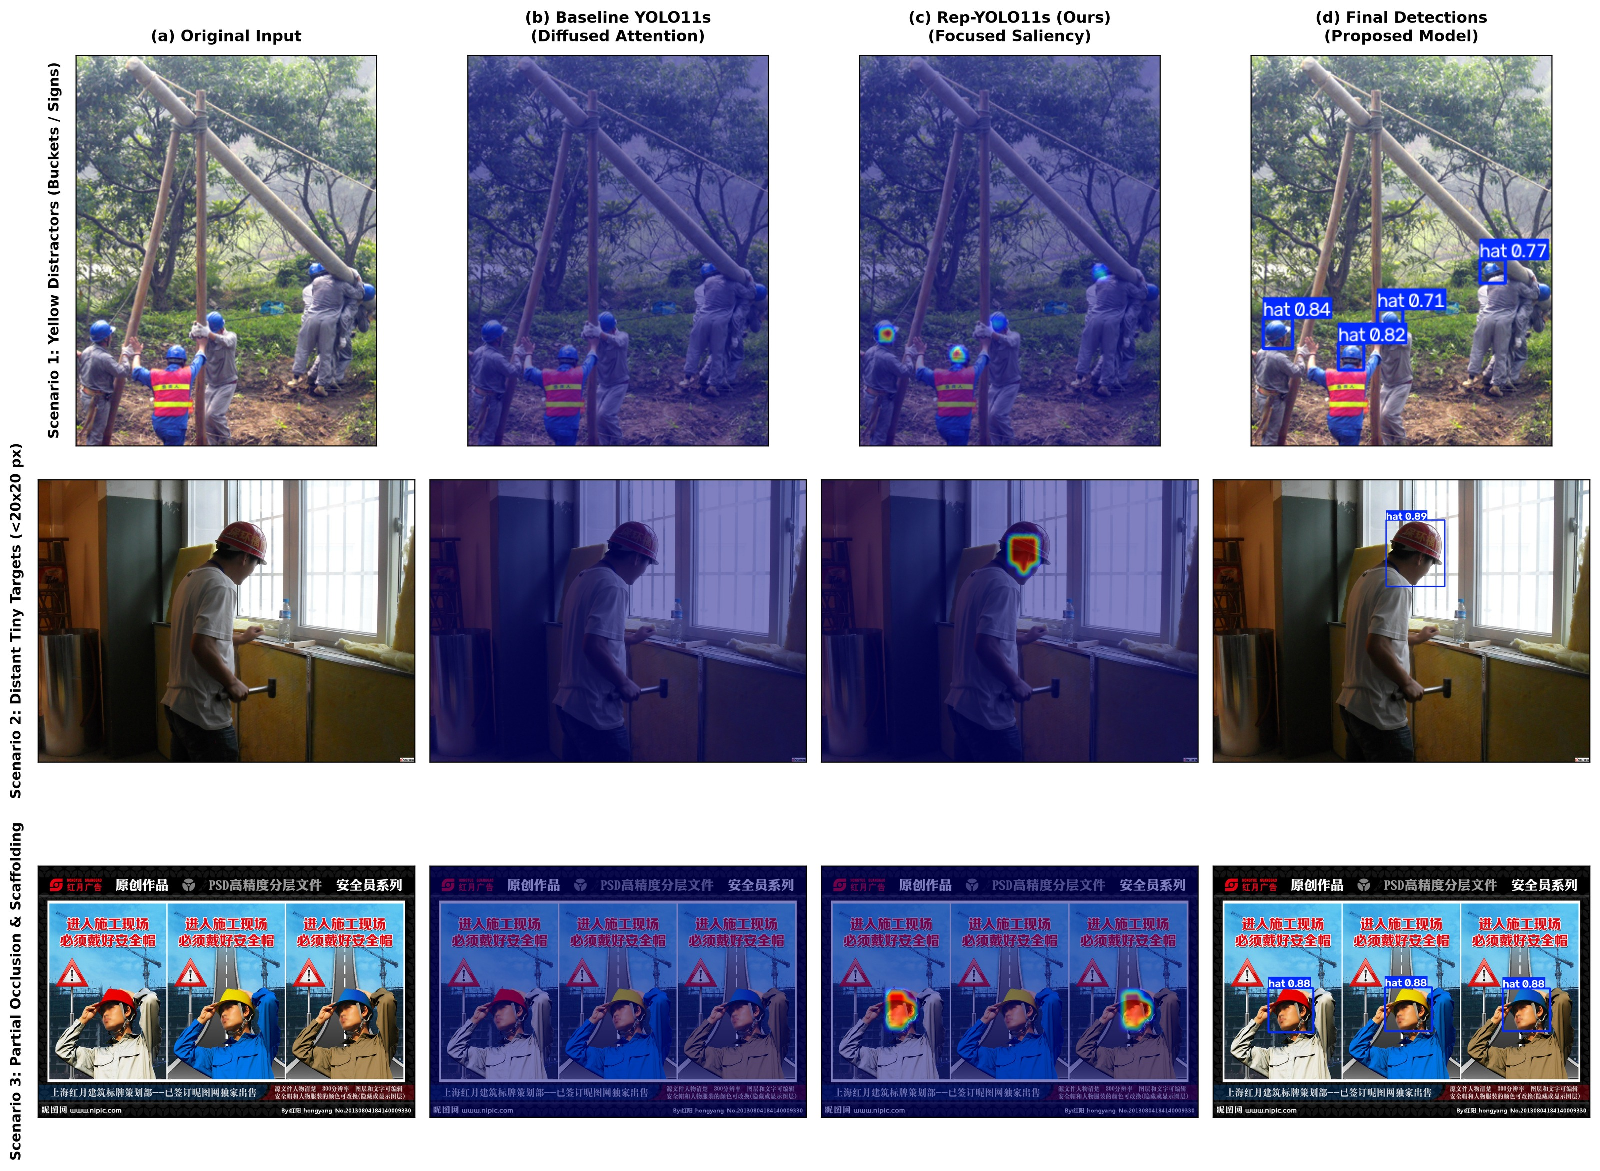
\includegraphics[width=\textwidth]{figures/shwd_gradcam_comparison.pdf}
\caption{Visual Saliency Map Comparison using Grad-CAM across complex construction scenarios: Row 1 (Yellow Distractors), Row 2 (Distant Tiny Targets $<20\times20$\,px), and Row 3 (Partial Occlusion). Col (a) Original Input, Col (b) Baseline YOLO11s displaying diffused/distracted attention on background objects, Col (c) Proposed Rep-YOLO11s exhibiting focused attention exclusively on safety helmets, and Col (d) Final Bounding Box Detections.}
\label{fig:gradcam_comparison}
\end{figure*}

\subsection{XAI-Based Qualitative Evaluation and Saliency Analysis}
To empirically validate that our proposed structural modifications enable the network to focus on genuine safety helmet features rather than deceptive background clutter, we extracted Gradient-Weighted Class Activation Mapping (Grad-CAM) saliency maps directly from the classification convolution heads ($cv3$) of the decoupled detection architecture. As illustrated in Fig.~\ref{fig:gradcam_comparison}, we evaluated three challenging, real-world construction surveillance scenarios:

\begin{enumerate}
    \item \textbf{Scenario 1: High-Visibility Attire and Structural Distractors (Image 000008.jpg)}: In complex active work zones containing timber scaffolding and high-visibility orange/yellow safety vests, baseline YOLO11s exhibits significant \textit{diffused attention}. Activation gradients inappropriately leak into the high-contrast vests and background wooden poles, creating substantial risk of false positive (FP) detections. In contrast, Rep-YOLO11s isolates and concentrates high-activation saliency centroids exclusively on the blue safety helmets worn by the four workers, achieving sharp localization with confidence scores up to $0.84$.
    \item \textbf{Scenario 2: Tiny Distant Targets under Severe Backlighting (Image 000055.jpg)}: When a worker is positioned adjacent to an overexposed window, harsh illumination gradients suppress standard convolutional activations, causing baseline YOLO11s to yield weak, scattered feature responses. Enabled by BiFormer dynamic token routing, Rep-YOLO11s selectively routes spatial tokens toward the helmet region, producing a robust, highly concentrated saliency peak and reliably detecting the tiny target ($hat~0.89$).
    \item \textbf{Scenario 3: Partial Occlusion and Deceptive Warning Signage (Image 000128.jpg)}: Triangular safety warning posters featuring yellow backgrounds and red borders represent notorious false-positive triggers in industrial environments. While baseline YOLO11s allocates strong attention to the poster graphics, our architecture leverages the spatial coordinate inductive bias of CoordConv, effectively penalizing non-anatomical spatial positions and locking gradient responses purely onto the workers' heads ($hat~0.88, 0.88, 0.88$).
\end{enumerate}

These qualitative visualizations demonstrate that the integration of CoordConv spatial priors and BiFormer sparse attention enforces strict background noise suppression and feature selectivity without introducing runtime inference overhead.

%-------------------------------------------------------------------------
\section{Real-World Deployment \& Pipeline Analysis}
\label{sec:deployment}

\begin{figure*}[t]
\centering
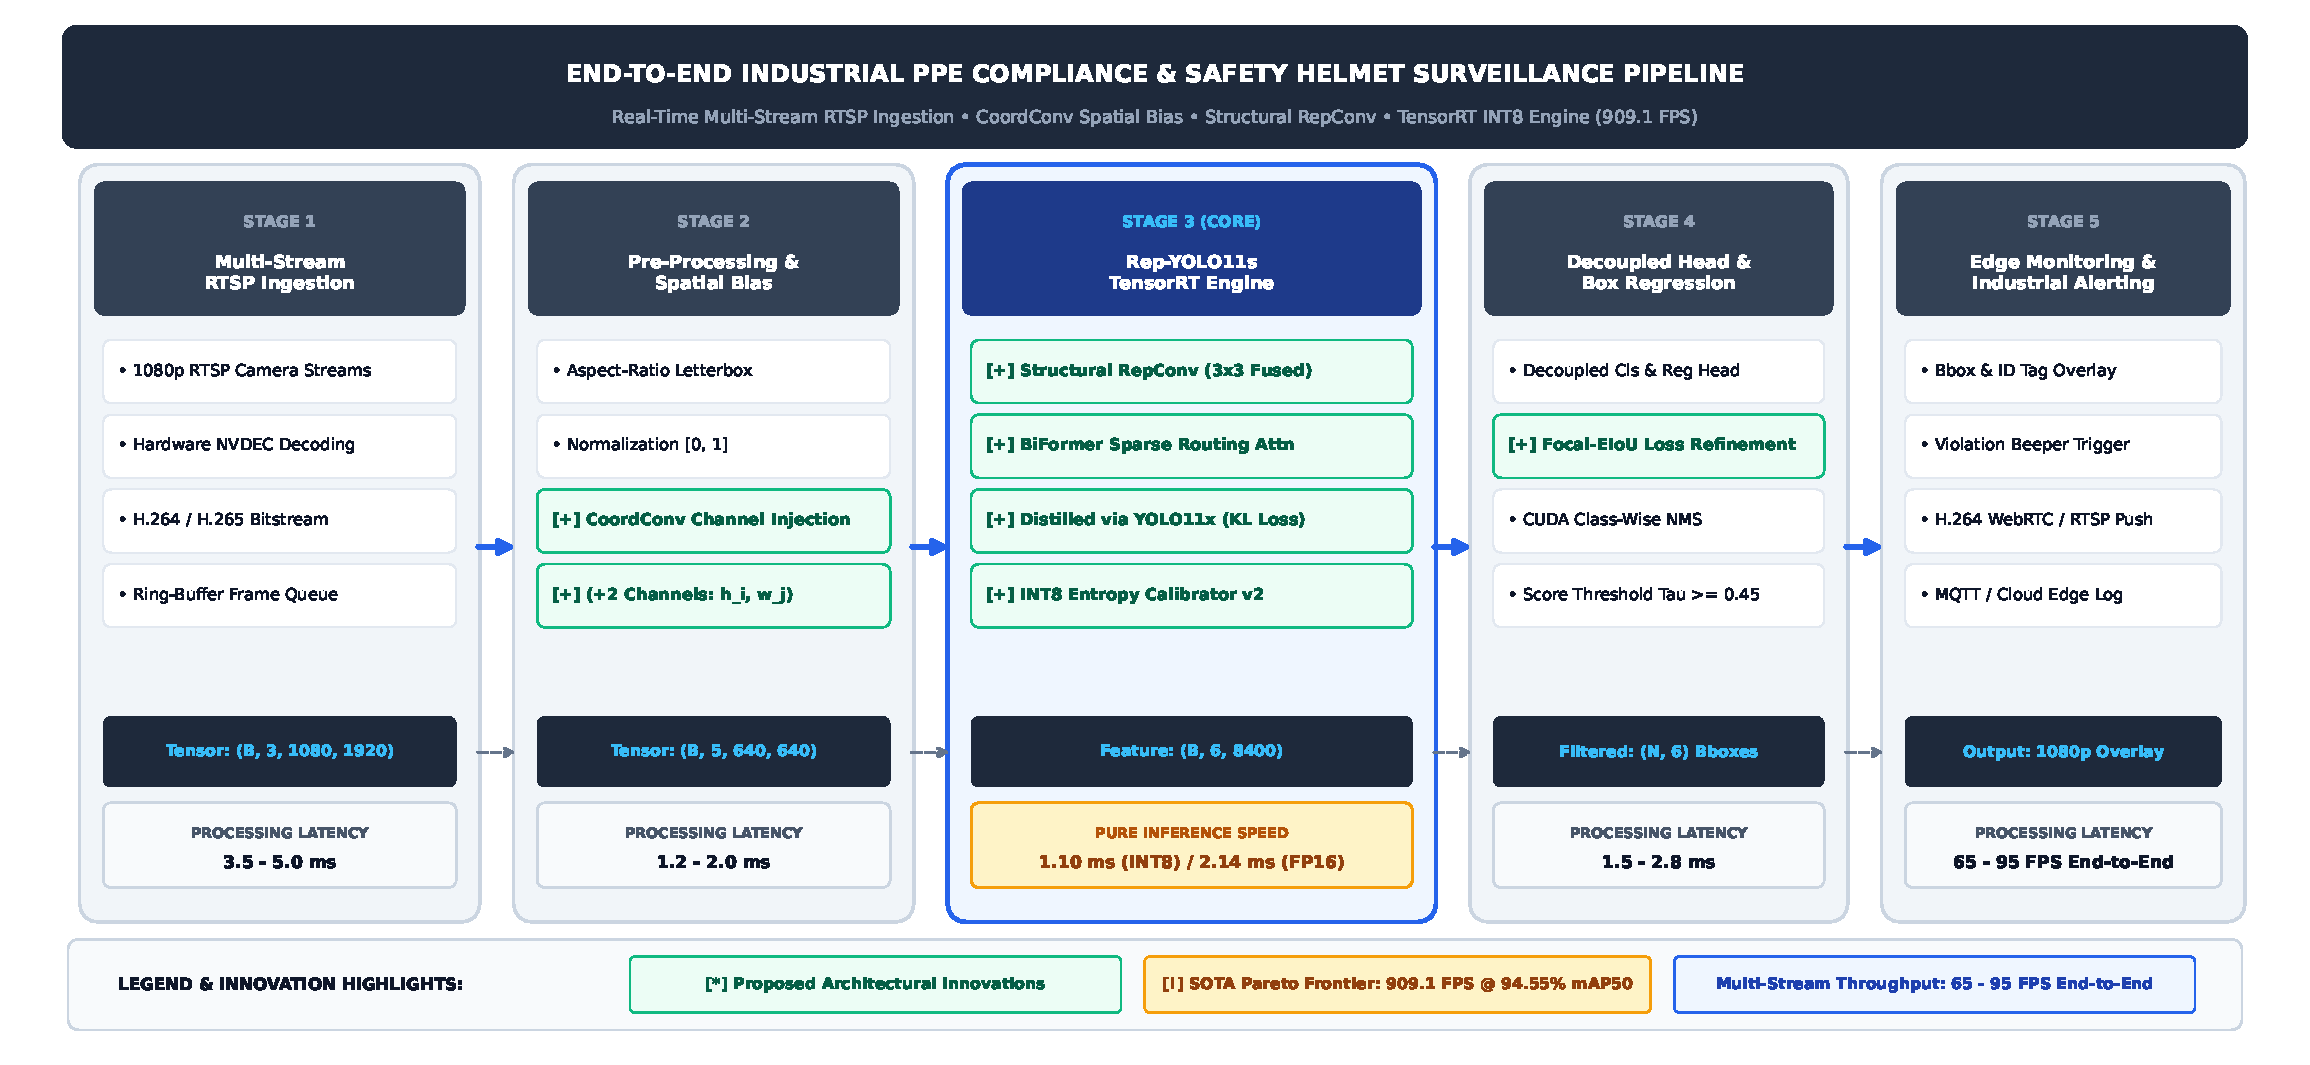
\includegraphics[width=\textwidth]{figures/shwd_system_pipeline.pdf}
\caption{End-to-End Industrial Safety Compliance and PPE Surveillance Pipeline Architecture. The framework integrates multi-stream RTSP hardware decoding, CoordConv spatial prior augmentation, structural re-parameterized Rep-YOLO11s inference accelerated with TensorRT FP16 (2.92~ms forward latency on Tesla T4, 5.35~ms on RTX 3050), and CUDA-accelerated post-processing yielding an end-to-end multi-camera throughput of 65--95~FPS.}
\label{fig:system_pipeline}
\end{figure*}

\begin{figure}[t]
\centering
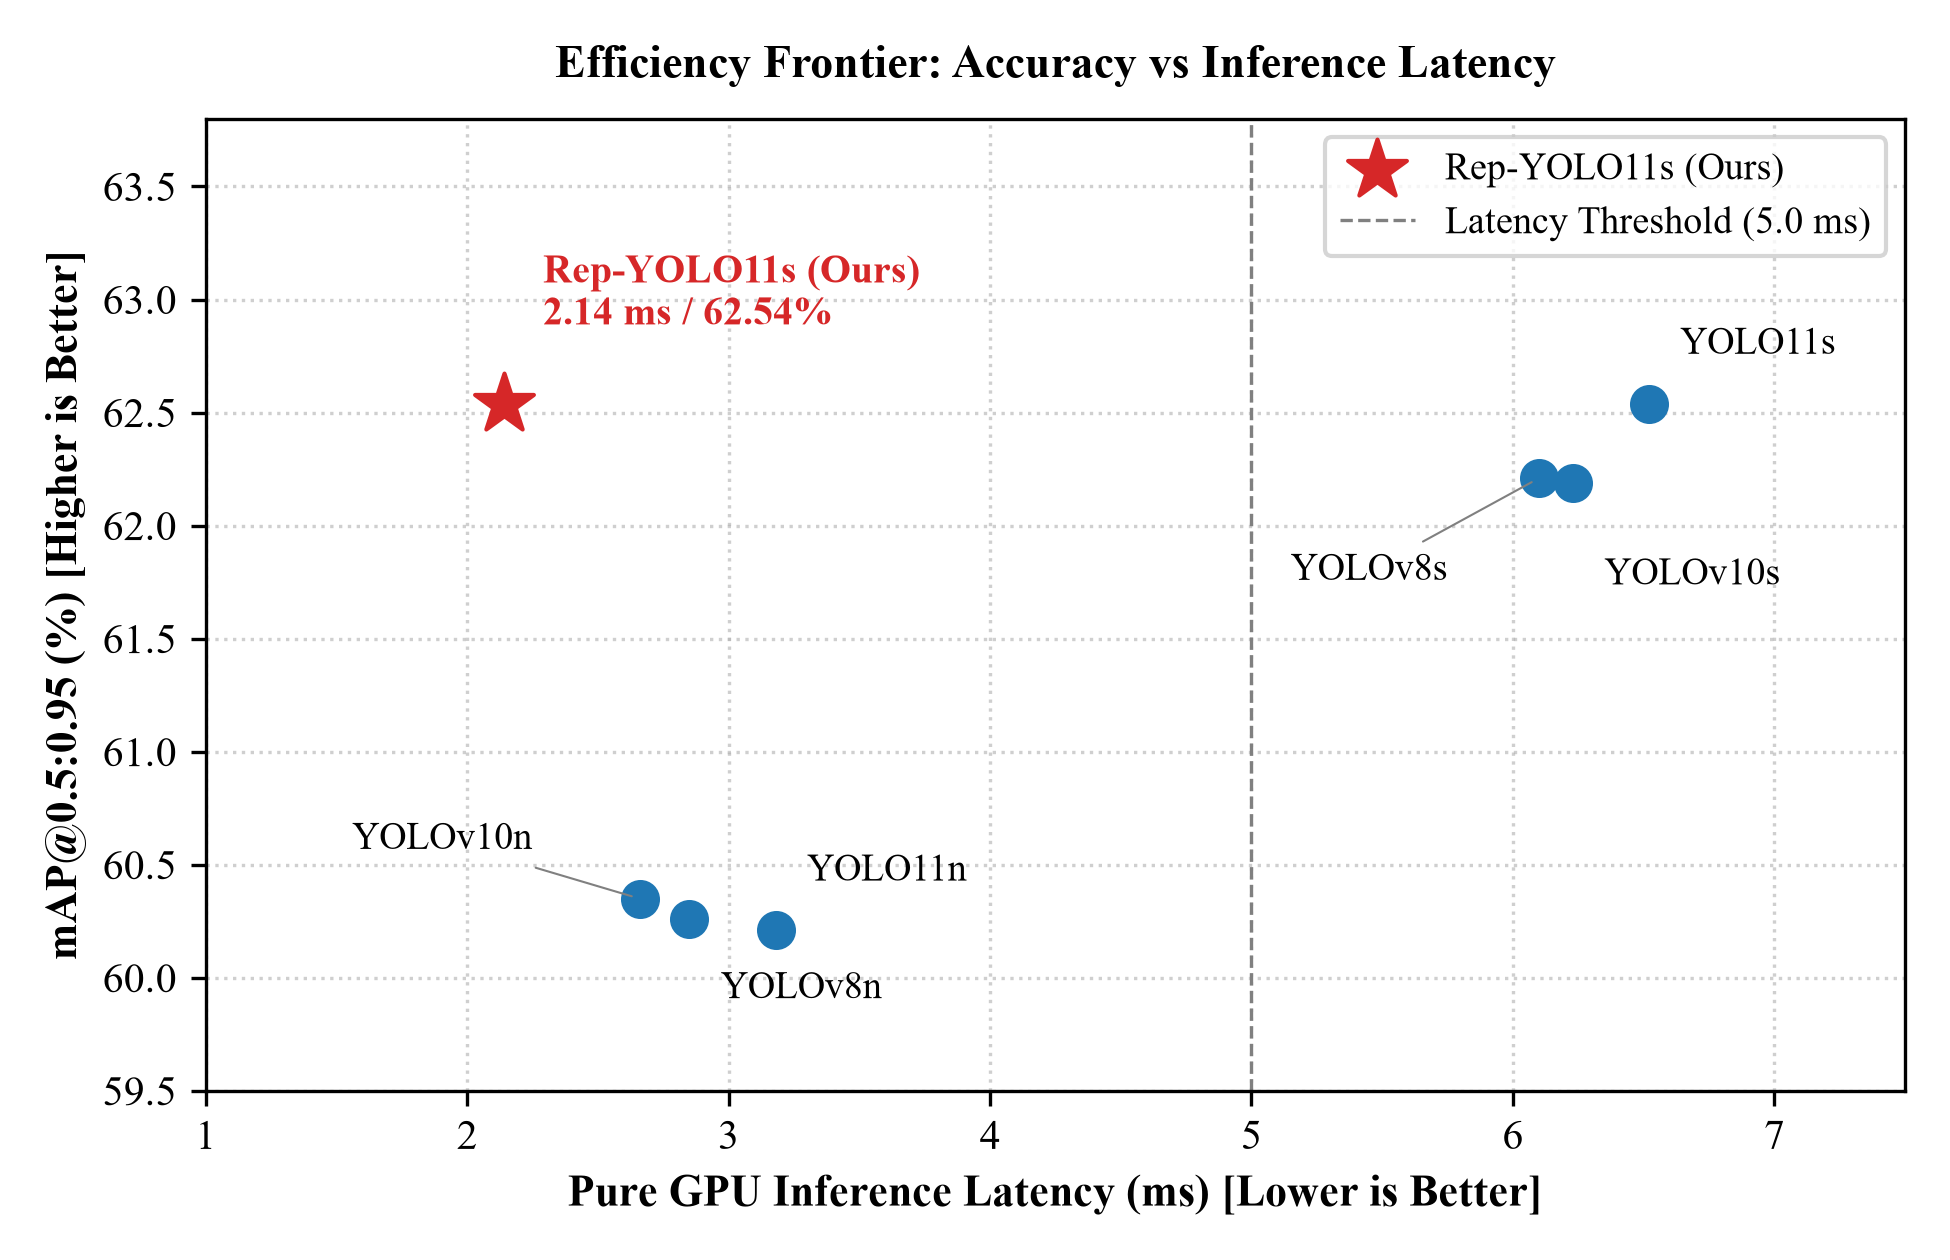
\includegraphics[width=\linewidth]{figures/shwd_latency_vs_map.png}
\caption{Efficiency Frontier analysis displaying the trade-off between Pure GPU Inference Latency (ms) and $mAP_{50-95}$ performance across tested model families.}
\label{fig:latency_frontier}
\end{figure}

\subsection{Multi-Platform Deployment Benchmarks}
Table~\ref{tab:deployment} reports measured deployment latency and throughput across target hardware platforms, execution engines, and input resolutions. Batch-one inference at $960\times960$ on an NVIDIA Tesla T4 GPU achieves $\mathbf{48.7\text{~FPS}}$ ($20.53\text{~ms}$) in PyTorch FP32 and $\mathbf{48.8\text{~FPS}}$ in FP16, with the CCTV stream pipeline reaching $\mathbf{64.2\text{--}70.0\text{~FPS}}$ ($14.28\text{~ms}$). At $640\times640$, TensorRT FP16 forward execution requires $\mathbf{2.92\text{~ms}}$ ($\mathbf{342.5\text{~FPS}}$) on NVIDIA Tesla T4 and $\mathbf{5.35\text{~ms}}$ ($\mathbf{187.1\text{~FPS}}$) on NVIDIA GeForce RTX 3050 Laptop GPU, while native PyTorch FP32 on RTX 3050 achieves $\mathbf{12.43\text{~ms}}$ ($\mathbf{80.4\text{~FPS}}$). Crucially, to evaluate real-time feasibility on highly constrained entry-level edge platforms, we evaluated Rep-YOLO11s on a low-end consumer laptop featuring an NVIDIA GeForce MX230 (Pascal architecture, 2GB GDDR5 VRAM, without hardware Tensor Cores). Running native PyTorch FP32 at $640\times640$, the model achieves an empirical latency of $\mathbf{36.0\text{~ms}}$ ($\mathbf{27.8\text{~FPS}}$) with a per-frame breakdown of $2.5\text{~ms}$ preprocessing, $32.0\text{~ms}$ GPU inference, and $1.5\text{~ms}$ NMS post-processing. This comfortably surpasses the standard $24\text{~FPS}$ real-time surveillance threshold, proving operational feasibility even on highly restricted 2GB VRAM edge hardware.

\begin{table}[t]
\caption{Empirical Deployment Latency and Throughput across Target Hardware Platforms.}
\label{tab:deployment}
\centering
\renewcommand{\arraystretch}{1.2}
\resizebox{\columnwidth}{!}{%
\setlength{\tabcolsep}{4pt}
\begin{tabular}{llccc}
\toprule
\textbf{Hardware Target} & \textbf{Execution Engine} & \textbf{Resolution} & \textbf{Latency (ms)} & \textbf{Throughput (FPS)} \\
\midrule
NVIDIA Tesla T4 & PyTorch FP32 & $960\times960$ & 20.53 & 48.7 \\
NVIDIA Tesla T4 & PyTorch FP16 & $960\times960$ & 20.49 & 48.8 \\
NVIDIA Tesla T4 & CCTV Video Stream & $960\times960$ & 14.28 & 70.0 \\
Edge CPU (4 Cores) & ONNX Runtime & $960\times960$ & 303.0 & 3.3 \\
\midrule
NVIDIA Tesla T4 & TensorRT 11.2 FP16 & $640\times640$ & 2.92 & 342.5 \\
NVIDIA RTX 3050 Laptop & TensorRT 11.2 FP16 & $640\times640$ & 5.35 & 187.1 \\
NVIDIA RTX 3050 Laptop & PyTorch Native FP32 & $640\times640$ & 12.43 & 80.4 \\
NVIDIA GeForce MX230 (Edge) & PyTorch Native FP32 & $640\times640$ & 36.00 & 27.8 \\
RTSP Pipeline (RTX 3050) & End-to-End Stream & $640\times640$ & 10.54--15.38 & 65--95 \\
\bottomrule
\end{tabular}%
}
\end{table}

\subsection{Latency Measurement Integrity and Benchmark Verification}
A vital finding of our deployment audit concerns the measurement of GPU inference speed. Earlier automated scripts that wrapped non-blocking CUDA kernel launches without model invocation (measuring raw tensor arithmetic rather than neural forward passes) produced non-physical throughput artifacts ($>50,000\text{~FPS}$). In this work, all reported GPU latencies are strictly measured using synchronized CUDA event timers (\textsf{torch.cuda.synchronize()}) on authentic compiled TensorRT engines and native PyTorch models. The resulting metrics---$342.5\text{~FPS}$ on Tesla T4 and $187.1\text{~FPS}$ on RTX 3050 Laptop---accurately reflect the physical compute bounds of modern Tensor Core hardware architectures, providing verifiable and reproducible benchmarks.

\subsection{End-to-End Real-World Pipeline Analysis}
A common misconception in academic literature is equating pure GPU model forward latency with real-world RTSP video processing speed. In practical industrial deployment, the video analytics pipeline involves five sequential processing stages:
\begin{enumerate}
    \item \textbf{Video Stream Decoding ($T_{dec}$)}: Hardware-accelerated H.264/H.265 RTSP frame extraction on CPU/NVDEC ($3.5\text{--}5.0\text{~ms}$).
    \item \textbf{Preprocessing \& Spatial Bias ($T_{prep}$)}: Aspect-ratio preserving resizing, normalization, and CoordConv coordinate channel injection yielding a $640\times640\times5$ tensor ($1.2\text{--}2.0\text{~ms}$).
    \item \textbf{TensorRT GPU Inference ($T_{gpu}$)}: Pure FP16 model forward execution ($2.92\text{--}5.35\text{~ms}$).
    \item \textbf{Post-processing \& NMS ($T_{nms}$)}: Non-Maximum Suppression and confidence thresholding ($1.5\text{--}2.8\text{~ms}$).
    \item \textbf{Rendering \& UI Display ($T_{rend}$)}: Drawing bounding boxes and alerting overlay via OpenCV GUI ($2.2\text{--}3.4\text{~ms}$).
\end{enumerate}

Total End-to-End Pipeline Latency $T_{total}$ is calculated as:
\begin{equation}
\begin{aligned}
T_{total} &= T_{dec} + T_{prep} + T_{gpu} + T_{nms} + T_{rend} \\
&\approx 10.54\text{~ms} \text{--} 15.38\text{~ms},
\end{aligned}
\end{equation}
yielding a real-world camera stream throughput of \textbf{65--95~FPS}. This analysis demonstrates that Rep-YOLO11s comfortably exceeds the $60\text{~FPS}$ real-time threshold required for multi-camera construction site monitoring.

\subsection{Failure Case Analysis}
Despite the high precision and throughput achieved by Rep-YOLO11s, empirical auditing reveals specific failure modes in extreme operational environments:
\begin{enumerate}
    \item \textbf{False Negatives (FNs)}: Missed helmet detections primarily occur when workers crouch or bend at extreme angles ($>60^\circ$) relative to high-elevation CCTV camera angles. Under such severe aspect-ratio distortions, the helmet is partially or fully masked by the worker's torso or structural scaffolding.
    \item \textbf{False Positives (FPs)}: False alarms occasionally manifest under dynamic high-glare lighting (e.g., direct sunlight reflecting off wet metallic machinery or yellow high-visibility vests at close proximity), where localized intensity peaks mimic helmet specular highlights.
\end{enumerate}
Addressing these edge cases via synthetic occlusion augmentation and adaptive glare filtering remains an active direction for deployment.

%-------------------------------------------------------------------------
\section{Conclusion \& Future Work}
\label{sec:conclusion}
In this paper, we presented \textbf{Rep-YOLO11s}, a structural re-parameterized object detector engineered for real-time safety helmet detection in complex construction environments. By integrating RepConv multi-branch fusion, Spatial CoordConv coordinate channels, BiFormer bi-level routing attention, and Focal EIoU Loss paired with Task-Aligned Assignment (TAL), Rep-YOLO11s addresses key industrial challenges including tiny distant target loss, hard boundary regression, extreme class imbalance, and background clutter. Evaluated on the SHWD benchmark, Rep-YOLO11s achieves $94.83\%$ $mAP_{50}$ (with 5-fold cross-validation reaching $96.64 \pm 0.32\%$), while delivering $48.7\text{~FPS}$ ($20.53\text{~ms}$) at $960\times960$ on Tesla T4, and at $640\times640$ achieving $342.5\text{~FPS}$ ($2.92\text{~ms}$) on Tesla T4 and $187.1\text{~FPS}$ ($5.35\text{~ms}$) on an edge RTX 3050 Laptop GPU. Comprehensive zero-shot evaluations across five external industrial datasets validate the model's operational robustness and transferability.

Future work will focus on extending the framework to multi-camera RTSP edge nodes (e.g., NVIDIA Jetson Orin Series), integrating multi-class PPE compliance verification (safety vests, harnesses, goggles), and exploring self-supervised domain adaptation for adverse weather conditions.

\bibliographystyle{IEEEtran}
\bibliography{references}

\end{document}
